\documentclass[tikz,border=10pt]{standalone}
\usepackage{tikz}

\begin{document}
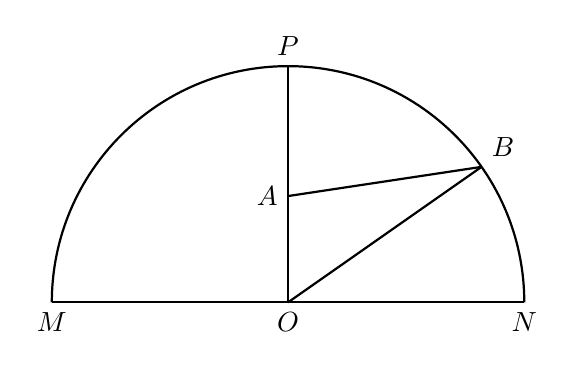
\begin{tikzpicture}[>=stealth, thick, scale=2]
    % 1. 定义基本参数
    \def\R{1.5}          % 半圆半径
    \def\thetaValue{35} % 点B相对于正右方的角度（弧度制或角度制调整）

    % 2. 定义关键点坐标
    \coordinate (O) at (0,0);                    % 圆心
    \coordinate (M) at (-\R, 0);                 % 左端点
    \coordinate (N) at (\R, 0);                  % 右端点
    \coordinate (P) at (0, \R);                  % 顶端点（垂直半径端点）
    \coordinate (A) at (0, 0.45*\R);              % OP上的动点A（设在OP约0.6倍距离处）
    \coordinate (B) at (\thetaValue:\R);        % 圆弧上的点B

    % 3. 绘制图形边界
    % 绘制半圆弧 MN，起点为 0度，终点为 180度
    \draw (N) arc (0:180:\R);
    
    % 绘制直径 MN
    \draw (M) -- (N);
    
    % 4. 绘制内部线段
    \draw (O) -- (P);      % 垂直半径 OP
    \draw (O) -- (B);      % 线段 OB
    \draw (A) -- (B);      % 线段 AB

    % 5. 标注文本（微调标注位置以防重叠）
    \node[below] at (O) {$O$};
    \node[below] at (M) {$M$};
    \node[below] at (N) {$N$};
    \node[above] at (P) {$P$};
    \node[left]  at (A) {$A$};
    \node[above right] at (B) {$B$};

\end{tikzpicture}
\end{document}